\documentclass[12pt,a4paper,oneside]{report}

\usepackage[margin=0.9in,top=0.9in,bottom=0.9in]{geometry}
\usepackage[utf8]{inputenc}
\usepackage{lmodern}
\usepackage{amsmath,amssymb}
\usepackage{booktabs}
\usepackage{array}
\usepackage{fancyhdr}
\usepackage{float}
\usepackage{graphicx}
\usepackage{xcolor}
\usepackage{hyperref}
\usepackage{titlesec}
\usepackage{tikz}
\usetikzlibrary{shapes.geometric,arrows.meta,positioning,calc,fit}

% -------------------------------------------------------------------------
% Page formatting
% -------------------------------------------------------------------------
\titleformat{\chapter}[display]
  {\normalfont\LARGE\bfseries}{\chaptertitlename\ \thechapter}{3pt}{\LARGE}
\titlespacing*{\chapter}{0pt}{-35pt}{12pt}
\titlespacing*{\section}{0pt}{10pt}{4pt}
\titlespacing*{\subsection}{0pt}{7pt}{3pt}

\pagestyle{fancy}
\fancyhf{}
\fancyhead[L]{\small\sffamily UCS503 - Software Engineering Project}
\fancyhead[R]{\small\sffamily SCMS Project Report}
\fancyfoot[C]{\thepage}
\renewcommand{\headrulewidth}{0.4pt}

\hypersetup{
    colorlinks=true,
    linkcolor=blue!60!black,
    citecolor=teal!60!black,
    urlcolor=blue!60!black
}

% -------------------------------------------------------------------------
% TikZ styles
% -------------------------------------------------------------------------
\tikzset{
    process/.style={
        rectangle, rounded corners=3pt, draw=blue!65!black,
        minimum width=3.5cm, minimum height=0.85cm,
        align=center, font=\sffamily\small\bfseries
    },
    store/.style={
        rectangle, draw=teal!65!black,
        minimum width=3.2cm, minimum height=0.75cm,
        align=center, font=\sffamily\small\bfseries
    },
    actor/.style={
        rectangle, rounded corners=3pt, draw=black!70,
        minimum width=2.8cm, minimum height=0.75cm,
        align=center, font=\sffamily\small\bfseries
    },
    usecase/.style={
        ellipse, draw=blue!65!black,
        minimum width=3.8cm, minimum height=0.75cm,
        align=center, font=\sffamily\small
    },
    arrow/.style={->,>=Stealth,thick},
    relation/.style={draw,thick}
}

\begin{document}

% =========================================================================
% TITLE PAGE
% =========================================================================
\begin{titlepage}
    \centering
    \vspace*{0.5cm}

    {\Large\bfseries UCS503 -- Software Engineering Project}\\[0.3cm]
    {\large Academic Year 2026--2027}\\[1.4cm]

    {\Huge\bfseries Sports Complex Management System (SCMS)}\\[0.5cm]
    {\large\textit{QR-Based Sports Equipment Booking, Fair Allocation and Inventory Management}}\\[1.8cm]

    {\large\textbf{Submitted by:}}\\[0.3cm]
    \begin{tabular}{ll}
        \textbf{1024240025} & Jaspreet Singh \\
        \textbf{1024240026} & Sanveer Singh \\
        \textbf{1024240028} & Harshjot Singh \\
    \end{tabular}\\[0.5cm]

    {\normalsize\textbf{B.E. Third Year, Computer Science \& Engineering}}\\[1.5cm]

    {\large\textbf{Submitted to:}}\\[0.2cm]
    {\large\textbf{Dr. Jeelani Asif}}\\[0.1cm]
    {\normalsize Department of Computer Science and Engineering}\\[1.2cm]

    \vfill
    {\normalsize\textbf{Software Engineering Project Report}}\\[0.15cm]
    {\normalsize\textbf{Computer Science and Engineering Department}}\\[0.1cm]
    {\normalsize Thapar Institute of Engineering and Technology, Patiala}\\[0.4cm]
\end{titlepage}

% =========================================================================
% TABLE OF CONTENTS
% =========================================================================
\pagenumbering{roman}
\tableofcontents
\newpage
\pagenumbering{arabic}

% =========================================================================
% CHAPTER 1
% =========================================================================
\chapter{Introduction}

\section{Background and Context}

Managing sports equipment in a university sports complex involves more than simply recording who borrowed an item. Students need to know equipment and slot availability, submit booking requests, receive fair allocation, and complete collection and return procedures. Staff need reliable verification, issue/return records, inventory visibility, and damage tracking. Administrators need control over equipment, booking slots, fairness rules, staff accounts, defaulters, and analytics.

The \textbf{Sports Complex Management System (SCMS)} is designed as a full-stack system for digitising this workflow. Students and staff use a Flutter mobile application, while administrators use a React web dashboard. A FastAPI backend provides the central business logic and connects the applications to a PostgreSQL database.

\section{Problem Statement}

Traditional or manually managed sports equipment booking can lead to several operational problems:

\begin{itemize}
    \item Lack of real-time visibility of equipment and slot availability.
    \item Manual handling of booking requests and allocation.
    \item Unequal access when many students request limited-capacity slots.
    \item Difficulty verifying students and equipment during issue and return.
    \item Incomplete tracking of overdue, damaged, or returned equipment.
    \item Limited visibility of usage statistics and operational performance.
\end{itemize}

SCMS addresses these problems through centralised booking, configurable fairness-based allocation, QR verification, transaction tracking, inventory management, notifications, and an administrative analytics dashboard.

\section{Project Objectives}

The major objectives of SCMS are:

\begin{enumerate}
    \item Provide students with a digital platform to browse equipment and available slots.
    \item Allow students to submit and track equipment booking requests.
    \item Allocate limited-capacity slots using a transparent fairness-based priority mechanism.
    \item Provide QR-based student and equipment verification for issue and return operations.
    \item Maintain a central inventory with equipment status and condition.
    \item Record every equipment issue and return as a transaction.
    \item Identify overdue users and maintain defaulter records.
    \item Provide in-app notifications for booking, waitlist, return, and overdue events.
    \item Provide administrators with inventory, bookings, transactions, defaulters, staff, fairness, and analytics management.
    \item Provide a deployable architecture that can be piloted with real-time sports-complex operations.
\end{enumerate}

\section{Scope}

The system covers three main user-facing interfaces:

\begin{itemize}
    \item \textbf{Student Mobile Application:} registration, login, equipment browsing, slot booking, booking status, QR identity, history, notifications, and profile.
    \item \textbf{Staff Mobile Application:} QR scanning, student validation, equipment issue, return processing, damage logging, queue viewing, and inventory status.
    \item \textbf{Admin Web Dashboard:} dashboard, analytics, inventory, slots, bookings, transactions, defaulters, fairness configuration, and staff management.
\end{itemize}

The backend is the single source of truth for authentication, authorisation, booking rules, fairness allocation, transactions, inventory state, notifications, and scheduled operations.

% =========================================================================
% CHAPTER 2
% =========================================================================
\chapter{Methodology and System Design}

\section{System Architecture}

SCMS follows a client-server architecture with separate interfaces for students, staff, and administrators. Both mobile and web clients communicate with a central FastAPI backend. The backend communicates with PostgreSQL for persistent data storage.

\begin{figure}[H]
\centering
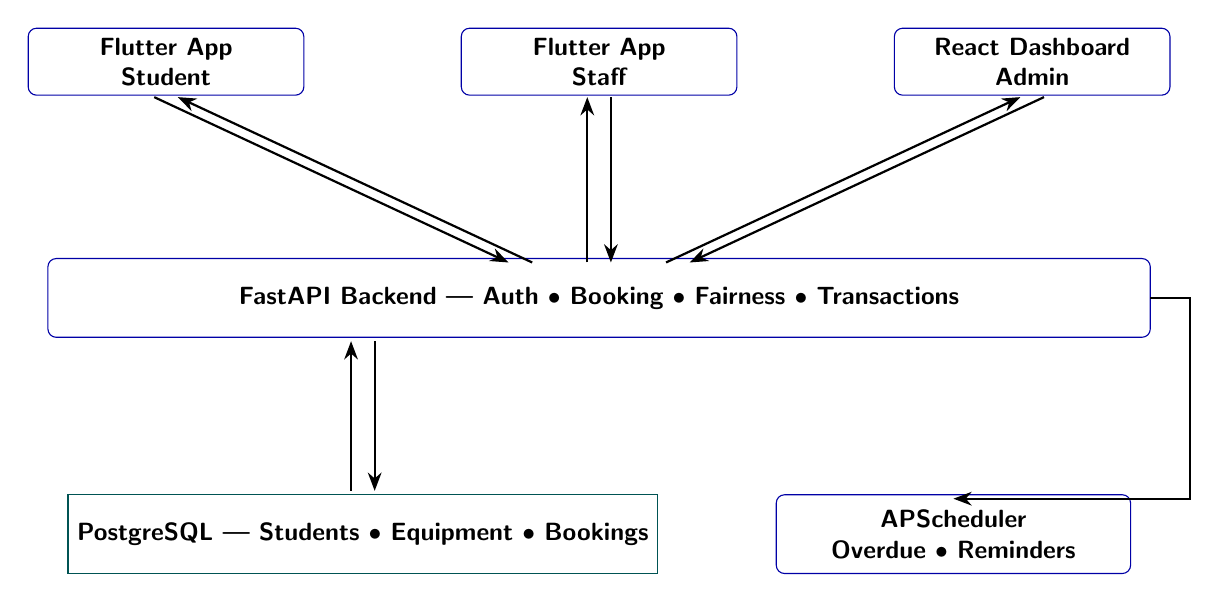
\begin{tikzpicture}[x=1cm, y=1cm]

%% Row 1 – three clients
%% student x=2, staff x=7.5, web x=13
%% width=3.5cm each => spans [0.25,3.75], [5.75,9.25], [11.25,14.75]
\node[process, minimum width=3.5cm] (student) at (2,    0) {Flutter App\\Student};
\node[process, minimum width=3.5cm] (staff)   at (7.5,  0) {Flutter App\\Staff};
\node[process, minimum width=3.5cm] (web)     at (13,   0) {React Dashboard\\Admin};

%% Row 2 – API centred x=7.5, width=14cm => spans [0.5, 14.5]
\node[process, minimum width=14cm, minimum height=1cm] (api) at (7.5, -3)
    {FastAPI Backend --- Auth $\bullet$ Booking $\bullet$ Fairness $\bullet$ Transactions};

%% Row 3 – DB centred x=4.5 width=7cm => [1, 8]
%%         Sched centred x=12 width=4.5cm => [9.75, 14.25]  gap=1.75cm
\node[store,   minimum width=7cm,   minimum height=1cm] (db)    at (4.5, -6)
    {PostgreSQL --- Students $\bullet$ Equipment $\bullet$ Bookings};
\node[process, minimum width=4.5cm, minimum height=1cm] (sched) at (12,  -6)
    {APScheduler\\Overdue $\bullet$ Reminders};

%% Student <-> API
\draw[arrow] (1.85, -0.45) -- (6.35, -2.55);
\draw[arrow] (6.65, -2.55) -- (2.15, -0.45);

%% Staff <-> API
\draw[arrow] (7.65, -0.45) -- (7.65, -2.55);
\draw[arrow] (7.35, -2.55) -- (7.35, -0.45);

%% Web <-> API
\draw[arrow] (13.15, -0.45) -- (8.65, -2.55);
\draw[arrow] ( 8.35, -2.55) -- (12.85, -0.45);

%% API <-> DB
\draw[arrow] (4.65, -3.55) -- (4.65, -5.45);
\draw[arrow] (4.35, -5.45) -- (4.35, -3.55);

%% API -> Scheduler: right elbow then down to sched.north
\draw[arrow] (14.5, -3) -- (15, -3) -- (15, -5.55) -- (12, -5.55);

\end{tikzpicture}
\caption{High-Level SCMS System Architecture}
\label{fig:architecture}
\end{figure}

\section{Technical Stack}

The project uses the following technologies:

\begin{table}[H]
\centering
\small
\begin{tabular}{p{3.3cm}p{9.2cm}}
\toprule
\textbf{Layer} & \textbf{Technology / Purpose}\\
\midrule
Mobile & Flutter 3, Dart, Riverpod, GoRouter, Dio\\
Web & React 18, TypeScript 5, Vite 5, TanStack Query, Axios\\
Backend & Python, FastAPI 0.115\\
Database & PostgreSQL, SQLModel 0.0.21\\
Migrations & Alembic 1.13\\
Authentication & JWT (HS256), secure password hashing\\
QR & qr\_flutter for QR display, mobile\_scanner for scanning\\
Storage & flutter\_secure\_storage for mobile authentication data\\
Scheduling & APScheduler 3.10\\
Charts & Recharts 2\\
Web UI & Tailwind CSS 3, Radix UI, Lucide\\
Testing & pytest, Vitest, flutter\_test\\
Deployment & Docker, nginx\\
\bottomrule
\end{tabular}
\caption{SCMS Technology Stack}
\label{tab:stack}
\end{table}

\section{Core Modules}

The backend is organised around the following modules:

\begin{enumerate}
    \item \textbf{Authentication:} Student registration/login, staff login, JWT validation, role-based access, and session restoration.
    \item \textbf{Students:} Student records, QR identity, status, and usage information.
    \item \textbf{Equipment and Inventory:} Equipment records, categories, quantities, status, condition, and administrative CRUD operations.
    \item \textbf{Slots:} Admin-created booking slots with capacity, timing, cutoff, and status.
    \item \textbf{Bookings:} Booking requests, confirmation, waitlisting, cancellation, queue position, and priority information.
    \item \textbf{Fairness Engine:} Batch allocation using recent usage and recency-based priority.
    \item \textbf{Transactions:} Equipment issue, return, damage recording, and transaction history.
    \item \textbf{Notifications:} In-app booking, waitlist, return, overdue, and damage notifications.
    \item \textbf{Analytics:} Booking trends, utilisation, equipment usage, damage statistics, and operational KPIs.
    \item \textbf{Scheduler:} Automated slot cutoffs, no-show detection, overdue detection, and return reminders.
\end{enumerate}

% =========================================================================
% CHAPTER 3
% =========================================================================
\chapter{Data Flow and Database Design}

\section{Context-Level Data Flow Diagram}

At the highest level, SCMS is treated as a single process interacting with external entities. The main external entities are Student, Staff, Admin, and the Notification Service.

\begin{figure}[H]
\centering
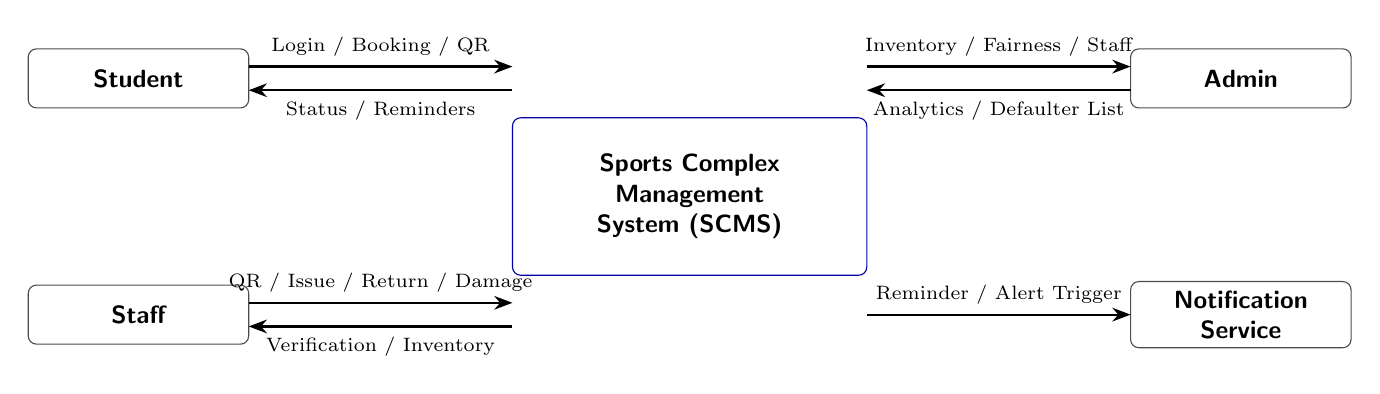
\begin{tikzpicture}[x=1cm, y=1cm]

%% Central SCMS process box -- wide enough, centred at (7, 0)
\node[process, minimum width=4.5cm, minimum height=2cm] (scms) at (7, 0)
    {Sports Complex\\Management\\System (SCMS)};

%% Actors -- well separated from SCMS
%% Left actors at x=0, right actors at x=14
\node[actor] (student) at (0,  1.5) {Student};
\node[actor] (staff)   at (0, -1.5) {Staff};
\node[actor] (admin)   at (14,  1.5) {Admin};
\node[actor] (notify)  at (14, -1.5) {Notification\\Service};

%% Student <-> SCMS
%% student.east is at (1.4, 1.5), scms.west is at (4.75, *)
\draw[arrow] (1.4, 1.65) -- node[above,font=\scriptsize]{Login / Booking / QR} (4.75, 1.65);
\draw[arrow] (4.75, 1.35) -- node[below,font=\scriptsize]{Status / Reminders}  (1.4,  1.35);

%% Staff <-> SCMS
\draw[arrow] (1.4, -1.35) -- node[above,font=\scriptsize]{QR / Issue / Return / Damage} (4.75, -1.35);
\draw[arrow] (4.75, -1.65) -- node[below,font=\scriptsize]{Verification / Inventory}    (1.4,  -1.65);

%% Admin <-> SCMS
%% scms.east is at (9.25, *), admin.west is at (12.6, 1.5)
\draw[arrow] (9.25, 1.65) -- node[above,font=\scriptsize]{Inventory / Fairness / Staff} (12.6, 1.65);
\draw[arrow] (12.6, 1.35) -- node[below,font=\scriptsize]{Analytics / Defaulter List}   (9.25, 1.35);

%% SCMS -> Notification (single arrow)
\draw[arrow] (9.25, -1.5) -- node[above,font=\scriptsize]{Reminder / Alert Trigger} (12.6, -1.5);

\end{tikzpicture}
\caption{Context-Level Data Flow Diagram}
\label{fig:context_dfd}
\end{figure}

\section{DFD Level 1}

The Level 1 DFD decomposes SCMS into its major internal processes:

\begin{itemize}
    \item \textbf{1.0 Registration \& Login}
    \item \textbf{2.0 Booking \& Scheduling}
    \item \textbf{3.0 Fairness Compute}
    \item \textbf{4.0 Issue/Return Transactions}
    \item \textbf{5.0 Inventory Management}
    \item \textbf{6.0 Notifications \& Analytics}
\end{itemize}

The principal data stores are Students (D1), Equipment Items (D2), Bookings (D3), Transactions (D4), Usage Statistics (D5), and Defaulters (D6).

\begin{figure}[H]
\centering
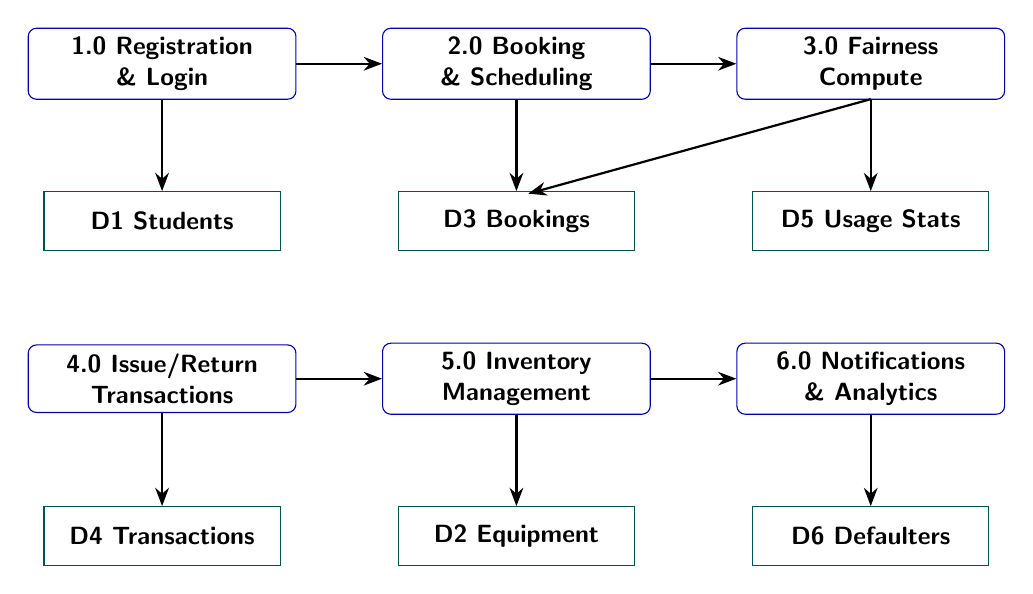
\begin{tikzpicture}[x=1cm,y=1cm]

% ---- Row 1 processes (y=0) ----
\node[process, minimum width=3.4cm] (p1) at (0,   0) {1.0 Registration\\\& Login};
\node[process, minimum width=3.4cm] (p2) at (4.5, 0) {2.0 Booking\\\& Scheduling};
\node[process, minimum width=3.4cm] (p3) at (9,   0) {3.0 Fairness\\Compute};

% ---- Row 2 stores (y=-2) ----
\node[store, minimum width=3cm] (d1) at (0,   -2) {D1 Students};
\node[store, minimum width=3cm] (d3) at (4.5, -2) {D3 Bookings};
\node[store, minimum width=3cm] (d5) at (9,   -2) {D5 Usage Stats};

% ---- Row 3 processes (y=-4) ----
\node[process, minimum width=3.4cm] (p4) at (0,   -4) {4.0 Issue/Return\\Transactions};
\node[process, minimum width=3.4cm] (p5) at (4.5, -4) {5.0 Inventory\\Management};
\node[process, minimum width=3.4cm] (p6) at (9,   -4) {6.0 Notifications\\\& Analytics};

% ---- Row 4 stores (y=-6) ----
\node[store, minimum width=3cm] (d4) at (0,   -6) {D4 Transactions};
\node[store, minimum width=3cm] (d2) at (4.5, -6) {D2 Equipment};
\node[store, minimum width=3cm] (d6) at (9,   -6) {D6 Defaulters};

% Row 1 process flows
\draw[arrow] (p1) -- (p2);
\draw[arrow] (p2) -- (p3);

% Row 3 process flows
\draw[arrow] (p4) -- (p5);
\draw[arrow] (p5) -- (p6);

% Process -> store (straight down)
\draw[arrow] (p1) -- (d1);
\draw[arrow] (p2) -- (d3);
\draw[arrow] (p3) -- (d5);
\draw[arrow] (p4) -- (d4);
\draw[arrow] (p5) -- (d2);
\draw[arrow] (p6) -- (d6);

% p3 -> d3  (diagonal, fairness writes back to bookings store)
\draw[arrow] (9, -0.45) -- (4.65, -1.65);

\end{tikzpicture}
\caption{DFD Level 1: Major SCMS Processes and Data Stores}
\label{fig:dfd1}
\end{figure}

\section{Entity Relationship Design}

The database is centred around students, equipment, bookings, transactions, usage statistics, and defaulters. The core relationships are:

\begin{itemize}
    \item A student \textbf{creates} bookings.
    \item A student \textbf{makes} transactions.
    \item A booking \textbf{reserves} an equipment item.
    \item A transaction records an equipment item being issued.
    \item A student \textbf{has} usage statistics.
    \item A student \textbf{may become} a defaulter.
\end{itemize}

\begin{figure}[H]
\centering
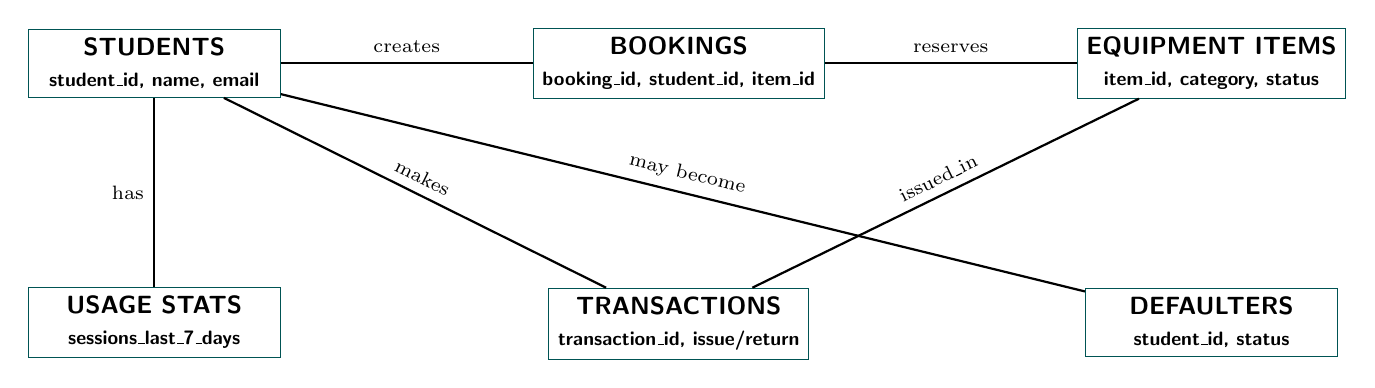
\begin{tikzpicture}[node distance=2.2cm and 2.8cm]

% Top row
\node[store] (students)   {STUDENTS\\\scriptsize student\_id, name, email};
\node[store, right=3.2cm of students] (bookings)
    {BOOKINGS\\\scriptsize booking\_id, student\_id, item\_id};
\node[store, right=3.2cm of bookings] (equipment)
    {EQUIPMENT ITEMS\\\scriptsize item\_id, category, status};

% Bottom row
\node[store, below=2.4cm of students]  (usage)
    {USAGE STATS\\\scriptsize sessions\_last\_7\_days};
\node[store, below=2.4cm of bookings]  (transactions)
    {TRANSACTIONS\\\scriptsize transaction\_id, issue/return};
\node[store, below=2.4cm of equipment] (defaulters)
    {DEFAULTERS\\\scriptsize student\_id, status};

% Relations
\draw[relation] (students)    -- node[above,font=\scriptsize]{creates}     (bookings);
\draw[relation] (bookings)    -- node[above,font=\scriptsize]{reserves}    (equipment);
\draw[relation] (students)    -- node[left,font=\scriptsize]{has}          (usage);
\draw[relation] (students)    -- node[above,sloped,font=\scriptsize]{makes}   (transactions);
\draw[relation] (transactions)-- node[above,sloped,font=\scriptsize]{issued\_in} (equipment);
\draw[relation] (students)    -- node[above,sloped,font=\scriptsize]{may become} (defaulters);

\end{tikzpicture}
\caption{Simplified Entity Relationship Design}
\label{fig:er}
\end{figure}

\section{Important Data Entities}

\subsection{Students}

Stores student identity and account information, including student ID, name, email, department, QR identity information, and account status.

\subsection{Equipment}

Stores equipment identity, category, quantity, status, and condition. Equipment states include \texttt{AVAILABLE}, \texttt{BOOKED}, \texttt{ISSUED}, \texttt{MAINTENANCE}, and \texttt{RETIRED}.

\subsection{Bookings}

Stores student booking requests, selected equipment/slot information, booking status, timing, and the priority score associated with allocation.

\subsection{Transactions}

Stores physical issue and return activity, including student, equipment, issue time, due time, return time, and return condition.

\subsection{Usage Statistics}

Stores recent student usage such as sessions and total minutes over the last seven days. These values support fairness calculation.

\subsection{Defaulters}

Stores active or resolved default records, including late-return information and current defaulter status.

% =========================================================================
% CHAPTER 4
% =========================================================================
\chapter{Functional Design and Workflows}

\section{Use Case Diagram}

The Use Case model identifies four actors: Student, Staff, Admin, and the System Notification Service.

\begin{figure}[H]
\centering
%% scale=0.56 shrinks the whole picture including text proportionally
\tikzset{uc/.style={ellipse, draw=blue!65!black,
    minimum width=4.2cm, minimum height=0.75cm,
    align=center, font=\sffamily\small}}
\scalebox{0.56}{%
\begin{tikzpicture}[x=1cm, y=1cm]

%% Actors
\node[actor, minimum width=2.8cm] (student) at (0,   4)  {Student};
\node[actor, minimum width=2.8cm] (staff)   at (0,  -9)  {Staff};
\node[actor, minimum width=2.8cm] (admin)   at (25,  4)  {Admin};
\node[actor, minimum width=2.8cm] (notify)  at (25, -9)  {Notification\\Service};

%% Student use cases  x=7
\node[uc] (login)        at (7,  8)   {Register / Login};
\node[uc] (availability) at (7,  6)   {View Equipment Availability};
\node[uc] (book)         at (7,  4)   {Book Equipment / Slot};
\node[uc] (status)       at (7,  2)   {View Booking Status};

%% Staff use cases  x=7
\node[uc] (scanstudent) at (7,  -5)  {Scan Student QR};
\node[uc] (issue)       at (7,  -7)  {Issue Equipment};
\node[uc] (return)      at (7,  -9)  {Process Return};
\node[uc] (damage)      at (7,  -11) {Log Damage};

%% Centre use cases  x=12.5
\node[uc] (priority) at (12.5, 0)   {Compute Priority Score};
\node[uc] (allocate) at (12.5, -2)  {Allocate Slot};

%% Admin use cases  x=18
\node[uc] (inventory) at (18,  8)   {Manage Equipment Inventory};
\node[uc] (analytics) at (18,  6)   {View Analytics Dashboard};
\node[uc] (defaulter) at (18,  4)   {View Defaulter List};
\node[uc] (fairness)  at (18,  2)   {Configure Fairness Rules};
\node[uc] (staffacct) at (18,  0)   {Manage Staff Accounts};

%% Notification use cases  x=18
\node[uc] (reminder) at (18,  -5)  {Send Return Reminder};
\node[uc] (overdue)  at (18,  -7)  {Flag Overdue};
\node[uc] (stats)    at (18,  -9)  {Update Usage Statistics};

%% Student lines
\draw[relation] (student) -- (login);
\draw[relation] (student) -- (availability);
\draw[relation] (student) -- (book);
\draw[relation] (student) -- (status);

%% Staff lines
\draw[relation] (staff) -- (scanstudent);
\draw[relation] (staff) -- (issue);
\draw[relation] (staff) -- (return);
\draw[relation] (staff) -- (damage);

%% Admin lines
\draw[relation] (admin) -- (inventory);
\draw[relation] (admin) -- (analytics);
\draw[relation] (admin) -- (defaulter);
\draw[relation] (admin) -- (fairness);
\draw[relation] (admin) -- (staffacct);

%% Notification lines
\draw[relation] (notify) -- (reminder);
\draw[relation] (notify) -- (overdue);
\draw[relation] (notify) -- (stats);

%% Include / extend (dashed)
\draw[relation,dashed] (book)
    -- node[above,font=\small]{$\langle\langle$include$\rangle\rangle$}
    (priority);
\draw[relation,dashed] (priority)
    -- node[right,font=\small]{$\langle\langle$include$\rangle\rangle$}
    (allocate);
\draw[relation,dashed] (return)
    -- node[above,font=\small]{$\langle\langle$include$\rangle\rangle$}
    (stats);
\draw[relation,dashed] (damage)
    -- node[right,font=\small]{$\langle\langle$extend$\rangle\rangle$}
    (return);

\end{tikzpicture}}
\caption{SCMS Use Case Diagram}
\label{fig:usecase}
\end{figure}

\section{Student Workflow}

The student workflow is:

\begin{enumerate}
    \item Register or log in.
    \item Browse available sports equipment.
    \item Select an available booking slot.
    \item Submit a booking request.
    \item Wait for the slot cutoff and fairness-based allocation.
    \item Receive a \texttt{CONFIRMED} or \texttt{WAITLISTED} result.
    \item View the booking and QR identity information.
    \item Collect the equipment through staff verification and QR scanning.
    \item Return the equipment through the staff-assisted return process.
    \item View transaction history and notifications.
\end{enumerate}

\section{Staff Workflow}

Staff performs the operational equipment-counter workflow:

\begin{enumerate}
    \item Open the staff queue or scan interface.
    \item Scan the student's QR code.
    \item Verify the student and confirmed booking.
    \item Scan the equipment QR code.
    \item Issue the equipment and create the transaction.
    \item When the equipment is returned, process the return.
    \item Record the equipment condition.
    \item If damaged, log the damage and place the equipment into maintenance.
\end{enumerate}

\section{Admin Workflow}

The administrator manages the overall system:

\begin{enumerate}
    \item Manage equipment inventory.
    \item Create and manage booking slots.
    \item Monitor bookings and transactions.
    \item Review defaulters.
    \item Configure fairness parameters.
    \item Manage staff/admin accounts.
    \item Monitor analytics and utilisation.
\end{enumerate}

\section{Booking and Allocation Workflow}

The booking lifecycle is:

\begin{center}
\texttt{REQUESTED}
$\rightarrow$
\texttt{CONFIRMED / WAITLISTED}
$\rightarrow$
\texttt{COMPLETED / CANCELLED / NO\_SHOW}
\end{center}

Allocation is performed in batch after the booking cutoff. Confirmed bookings occupy the available slot capacity; remaining eligible requests are waitlisted.

If a confirmed booking is cancelled or becomes a no-show, the next eligible waitlisted booking can be promoted.

% =========================================================================
% CHAPTER 5
% =========================================================================
\chapter{Fairness, Business Rules and Security}

\section{Fairness-Based Allocation}

SCMS uses a configurable fairness mechanism to avoid repeatedly favouring students who have already received substantial recent usage.

The priority score is:

\[
\boxed{Priority\ Score = S_{norm} + P_{recency}}
\]

where:

\[
S_{norm} =
\frac{\text{sessions in last 7 days}}
{\max(\text{sessions in last 7 days across students})}
\]

The recency component is:

\[
P_{recency} =
\begin{cases}
(2-d)\times 0.5, & d<2\\
0, & d\geq2
\end{cases}
\]

where $d$ represents the number of days since the student's last session.

A \textbf{lower score receives higher allocation priority}. This means the algorithm considers both recent usage and recency while maintaining a configurable daily usage cap.

\section{Daily Usage Cap}

The default daily cap is:

\[
\boxed{2\text{ sessions per student per day}}
\]

The value is configurable by an administrator. Students who reach the applicable cap are not allocated additional sessions under the fairness rules.

\section{Equipment State Management}

Equipment follows controlled states:

\begin{center}
\texttt{AVAILABLE}
$\rightarrow$
\texttt{BOOKED}
$\rightarrow$
\texttt{ISSUED}
$\rightarrow$
\texttt{AVAILABLE}
\end{center}

If returned damaged:

\begin{center}
\texttt{ISSUED}
$\rightarrow$
\texttt{RETURNED\_DAMAGED}
$\rightarrow$
\texttt{MAINTENANCE}
\end{center}

This prevents damaged equipment from being immediately issued again.

\section{No-Show and Overdue Rules}

A confirmed booking can be marked as \texttt{NO\_SHOW} if no transaction is recorded within the defined no-show window after the slot begins.

The scheduler also identifies overdue transactions and creates the relevant reminder or overdue records.

An active defaulter is prevented from creating a new booking according to the business rules. Defaulter status is separate from the administrative student status; becoming a defaulter does not automatically mean the student account is suspended.

\section{QR-Based Verification}

SCMS uses QR codes for operational verification.

The staff workflow verifies:

\begin{enumerate}
    \item Student identity.
    \item Booking eligibility.
    \item Equipment identity.
    \item Issue/return transaction.
\end{enumerate}

This reduces manual entry and links the physical equipment operation directly to the digital transaction record.

\section{Authentication and Authorisation}

Authentication uses JWT-based sessions with secure password hashing. The backend enforces role-based access so that:

\begin{itemize}
    \item Students can access student resources.
    \item Staff can access operational issue/return resources.
    \item Admins can access administrative management resources.
\end{itemize}

The backend remains the authority for permissions; the mobile or web interface does not independently decide whether an operation is allowed.

% =========================================================================
% CHAPTER 6
% =========================================================================
\chapter{Implementation and Interface Design}

\section{Student Mobile Application}

The student application is built using Flutter with Riverpod for state management and GoRouter for navigation.

The major student screens are:

\begin{table}[H]
\centering
\small
\begin{tabular}{p{3.4cm}p{9cm}}
\toprule
\textbf{Screen} & \textbf{Purpose}\\
\midrule
Splash & Restores the authentication session and routes the user.\\
Login & Student/staff credential entry.\\
Register & New student registration.\\
Home & Upcoming bookings and notification status.\\
Equipment & Browse available equipment.\\
Equipment Detail & View equipment details, choose slot, and book.\\
My QR & Display the student's QR identity.\\
Bookings & View active bookings and statuses.\\
Booking Detail & View booking details, queue position, and cancellation.\\
History & View completed transactions.\\
Transaction Detail & View issue/return details and condition.\\
Notifications & View read/unread in-app notifications.\\
Profile & View account information and usage statistics.\\
\bottomrule
\end{tabular}
\caption{Student Mobile Application Screens}
\label{tab:student_screens}
\end{table}

\section{Staff Mobile Application}

The staff interface provides the operational workflow:

\begin{table}[H]
\centering
\small
\begin{tabular}{p{3.4cm}p{9cm}}
\toprule
\textbf{Screen} & \textbf{Purpose}\\
\midrule
Staff Home & Today's queue and open transactions.\\
Scan & QR camera for operational scanning.\\
Student Validation & Verify student and booking after scanning.\\
Issue Confirmation & Confirm equipment issue.\\
Return Process & Process return and record condition/damage.\\
Queue & View confirmed bookings and open transactions.\\
Inventory & View equipment status.\\
Profile & Staff account and logout.\\
\bottomrule
\end{tabular}
\caption{Staff Mobile Application Screens}
\label{tab:staff_screens}
\end{table}

\section{Admin Web Dashboard}

The web dashboard is built using React, TypeScript, Vite, TanStack Query, Axios, Tailwind CSS, Radix UI, Recharts, and Lucide icons.

\begin{table}[H]
\centering
\small
\begin{tabular}{p{3.4cm}p{9cm}}
\toprule
\textbf{Screen} & \textbf{Purpose}\\
\midrule
Login & Staff/admin authentication.\\
Dashboard & Operational KPI summary and quick actions.\\
Analytics & Trends, utilisation, peak hours, and damage statistics.\\
Inventory & Equipment CRUD and status management.\\
Slots & Create/manage booking slots, capacity, and cutoffs.\\
Bookings & Review, filter, inspect, and cancel bookings.\\
Transactions & Review issue and return transactions.\\
Defaulters & Review and resolve defaulter records.\\
Fairness & Configure daily cap and fairness parameters.\\
Staff & Create, edit, and deactivate staff/admin accounts.\\
\bottomrule
\end{tabular}
\caption{Admin Web Dashboard Screens}
\label{tab:web_screens}
\end{table}

% =========================================================================
% CHAPTER 7
% =========================================================================
\chapter{Testing and Evaluation}

\section{Testing Strategy}

Testing was performed separately for the backend, web dashboard, and Flutter application.

\begin{enumerate}
    \item \textbf{Backend Unit and Integration Testing:} API, authentication, booking, fairness, transaction, inventory, notification, and scheduler behaviour.
    \item \textbf{Web Testing:} Component and page-level tests using Vitest and Testing Library.
    \item \textbf{Flutter Testing:} Widget/application tests together with static analysis.
    \item \textbf{Build Verification:} Production web build and Android debug APK build verification.
    \item \textbf{Runtime Verification:} Local PostgreSQL database, Alembic migrations, seeded demo data, backend API, and web dashboard integration.
\end{enumerate}

\section{Verification Results}

The current implementation has been verified using the following project-level results:

\begin{table}[H]
\centering
\small
\begin{tabular}{p{4.2cm}p{3.2cm}p{5.2cm}}
\toprule
\textbf{Component} & \textbf{Result} & \textbf{Verification}\\
\midrule
Backend & 26/26 tests passed & pytest suite green\\
Web Dashboard & 69/69 tests passed & Vitest suite green\\
Web TypeScript & 0 errors & Type checking successful\\
Web Production Build & Successful & Vite build completed\\
Flutter & 28/28 tests passed & flutter test suite green\\
Flutter Static Analysis & 0 issues & flutter analyze successful\\
Database Migration & Successful & Alembic initial schema applied\\
Demo Data & Successful & Seed data inserted and verified\\
\bottomrule
\end{tabular}
\caption{SCMS Verification Summary}
\label{tab:verification}
\end{table}

\section{Local End-to-End Environment}

The local deployment consists of:

\begin{itemize}
    \item PostgreSQL database for persistent storage.
    \item FastAPI backend running on port 8000.
    \item React web dashboard running through Vite during development.
    \item Flutter application connected to the backend using the appropriate local/emulator base URL.
    \item Alembic for database schema migration.
    \item Seed data for demonstrating the booking and fairness workflow.
\end{itemize}

A representative fairness demonstration uses a capacity-one slot with students having different recent usage. The fairness engine assigns the lower priority score to the student with greater allocation priority and places the other eligible request on the waitlist.

\section{Testing of Critical Business Scenarios}

The following scenarios are important for acceptance testing:

\begin{enumerate}
    \item Student registration and login.
    \item Student equipment and slot browsing.
    \item Booking request creation.
    \item Fairness-based confirmation and waitlisting.
    \item Booking cancellation and waitlist promotion.
    \item Student QR verification by staff.
    \item Equipment QR verification and issue.
    \item Normal return and equipment availability update.
    \item Damaged return and maintenance status update.
    \item Overdue detection and defaulter creation.
    \item In-app notification generation.
    \item Admin inventory, booking, transaction, fairness, and analytics operations.
\end{enumerate}

% =========================================================================
% CHAPTER 8
% =========================================================================
\chapter{Current Status, Deployment and Future Work}

\section{Current Implementation Status}

The project currently has the following implementation status:

\begin{table}[H]
\centering
\small
\begin{tabular}{p{5cm}p{6.8cm}}
\toprule
\textbf{Area} & \textbf{Status}\\
\midrule
Backend & Complete; routers, services, scheduler, migrations, and tests implemented.\\
Web Dashboard & Complete; administrative screens and analytics implemented.\\
Student Flutter App & Complete; student workflow and screens implemented.\\
Staff Flutter App & Complete; staff operational workflow implemented.\\
Automated Testing & All current project suites green.\\
Docker Deployment & Dockerfile and docker-compose prepared for deployment.\\
Real-Time Sports Complex Pilot & Next major step: deployment with institutional infrastructure and real operational data.\\
\bottomrule
\end{tabular}
\caption{Current SCMS Implementation Status}
\label{tab:status}
\end{table}

\section{Deployment Requirements}

Before production deployment, the following configuration steps are required:

\begin{enumerate}
    \item Configure a strong production \texttt{SECRET\_KEY}.
    \item Configure the production PostgreSQL database.
    \item Run the Alembic migrations using \texttt{alembic upgrade head}.
    \item Configure production CORS origins.
    \item Set the backend environment to production.
    \item Configure the Flutter application to use the production HTTPS backend URL.
    \item Deploy the web dashboard behind nginx or the selected production reverse proxy.
    \item Create controlled administrator and staff accounts.
\end{enumerate}

\section{Future Work}

The immediate next phase is a controlled pilot deployment at the Thapar Sports Complex. The pilot can validate the system using real equipment, slots, students, staff operations, and transaction data.

Future enhancements may include:

\begin{enumerate}
    \item Production cloud deployment and monitoring.
    \item Push notifications in addition to the current in-app notification mechanism.
    \item More detailed operational and usage analytics.
    \item Additional sports and resource categories.
    \item Integration with institutional authentication or student systems where permitted.
    \item Improved reporting and export facilities.
    \item Operational feedback-driven refinements after the initial sports-complex pilot.
\end{enumerate}

% =========================================================================
% CHAPTER 9
% =========================================================================
\chapter{Conclusion}

\section{Summary of Work}

The \textbf{Sports Complex Management System (SCMS)} provides an integrated digital workflow for sports equipment management. The system connects students, staff, administrators, and notification functionality through a common FastAPI backend and PostgreSQL database.

The project combines:

\begin{itemize}
    \item Digital equipment and slot booking.
    \item Fairness-based batch allocation.
    \item QR-based identity and equipment verification.
    \item Issue and return transaction management.
    \item Inventory and damage management.
    \item Overdue and defaulter handling.
    \item In-app notifications.
    \item Administrative analytics and management.
\end{itemize}

\section{Key Contribution}

The main contribution of SCMS is the integration of the \textbf{booking, fairness, physical issue/return, inventory, and administrative management workflows} into a single system. Instead of treating booking and equipment handling as separate processes, the system connects the complete lifecycle from a student's request to final equipment return.

\section{Final Remarks}

SCMS has reached a functional and tested state suitable for a controlled real-time pilot. The next stage is to work with the Thapar Sports Complex administration to configure institutional infrastructure, validate operational requirements, and deploy the system in a controlled environment.

% =========================================================================
% BIBLIOGRAPHY
% =========================================================================
\begin{thebibliography}{99}

\bibitem{fastapi}
FastAPI Documentation, ``FastAPI: Modern, Fast Web Framework for Building APIs with Python,'' 2026.

\bibitem{flutter}
Flutter Documentation, ``Flutter: Build apps for any screen,'' 2026.

\bibitem{react}
React Documentation, ``React: The library for web and native user interfaces,'' 2026.

\bibitem{postgresql}
PostgreSQL Documentation, ``PostgreSQL: The World's Most Advanced Open Source Relational Database,'' 2026.

\bibitem{alembic}
Alembic Documentation, ``Database Migration Tool for SQLAlchemy,'' 2026.

\bibitem{sqlmodel}
SQLModel Documentation, ``SQL databases in Python, designed for simplicity, compatibility, and robustness,'' 2026.

\bibitem{scms}
J.~Singh, S.~Singh, and H.~Singh, ``Sports Complex Management System (SCMS),'' Thapar Institute of Engineering and Technology, Software Engineering Project, 2026.

\end{thebibliography}

\end{document}
